%!TEX root = htm.tex
\section{Hybrid transactional memory algorithms}\label{sec:hytmalgos}
%
\begin{figure*}[!ht]
\begin{center}
	\subfloat[\label{sfig:ob-01}]{\scalebox{0.5}[0.5]{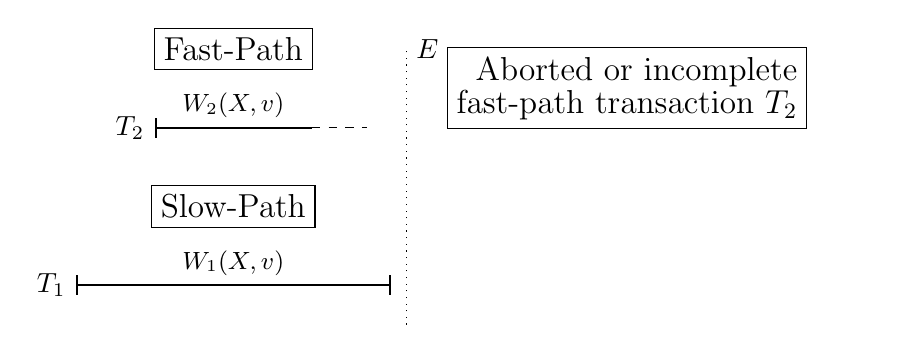
\begin{tikzpicture}
\node (w2) at (10,0) [] {};
\node (w1) at (10,-2) [] {};
\node (w3) at (18,-2) [] {};


\draw (w2) node [above] {\small {$W_2(X,v)$}};

\draw (w1) node [above] {\small {$W_1(X,v)$}};
%\draw (w1) node [below] {\tiny {$T_1$ commits}};


\node[draw,align=left] at (10,1) {{\large Fast-Path}};
\node[draw,align=left] at (10,-1) {{\large Slow-Path}};

\begin{scope}   
\draw [|-,thick] (9,0) node[left] {$T_2$} to (11,0);
\draw [-,dashed] (11,0) to (11.7,0);
\draw [|-|,thick] (8,-2) node[left] {$T_1$} to (12,-2);
\draw [-,dotted] (12.2,-2.5)  to (12.2,1) node[right] {$E$};
\end{scope}
%
\node[draw,align=right] at (15,.5) {\large {Aborted or incomplete}\\ {\large fast-path transaction $T_2$}};

%
\end{tikzpicture}
}}
	\hspace{10mm}
	\subfloat[\label{sfig:ob-02}]{\scalebox{0.5}[0.5]{\begin{tikzpicture}

\node (w1) at (11,-2) [] {};


\draw (w1) node [below] {\small {$W_1(X,v)$}};
%\draw (w1) node [below] {\tiny {$T_1$ commits}};

\node[draw,align=left] at (7,-2) {{\large Slow-Path}};

\begin{scope}   
\draw [|-|,thick] (9,-2) node[left] {$T_1$} to (13,-2);
\draw [-,dotted] (13.2,-2.5)  to (13.2,1) node[right] {$E'$};
\end{scope}
%
%
\end{tikzpicture}
}}
	 
\end{center}
\caption{
\label{fig:ob1}
Execution $E$ in Figure~\ref{sfig:ob-01} is indistinguishable
to $T_1$ from the execution $E'$ in Figure~\ref{sfig:ob-02}}
\end{figure*}
%
In this section, we first identify some invariants that follow from the HyTM execution model presented in the previous section.
We then describe two HyTM implementations: \cref{sec:hytm1} describes a progressive opaque TM while \cref{sec:hytm2} describes an opaque HyTM that is progressive only for read-only slow-path transactions.

Let $E$ be any execution of a HyTM implementation $\mathcal{M}$ in
which a fast-path transaction $T_k$ is either
t-incomplete or aborted. Let $E'$ be the execution fragment that is a subsequence of $E$ derived by removing all cached events of $E|k$.
%
\begin{observation} 
\label{ob:one}
To every slow-path transaction $T_m \in \ms{txns}(E)$, $E$ is indistinguishable from $E'$. Additionally, if a fast-path transaction $T_m\in \ms{txns}(E) \setminus \{T_k\}$ does not incur a tracking set abort in $E$, 
then $E$ is indistinguishable to $T_m$ from $E'$.
\end{observation}
%
%
%%%%%%%%%%%%%%%%%%%%%%%%%%%%%%%%%%%%%%%%%%%%%%%%%%%%%%%%%%%%%%%%%%%%%
%!TEX root = htm.tex
In this section, we present opaque HyTM algorithms that are progressive for a subset of transactions.

\vspace{1mm}\noindent\textbf{Instrumentation-optimal progressive HyTM.}
We describe a HyTM algorithm that is a tight bound for Theorem~\ref{th:impossibility} and the instrumentation cost on the fast-path transactions established in \cite{hytm14disc}.
For every t-object $X_j$, our implementation maintains a base object $v_j$ that stores the value of $X_j$
and a \emph{sequence lock} $r_{j}$. The sequence lock is an unsigned integer whose LSB bit stores the \emph{locked} state.
Specifically, we say that process $p_i$ \emph{holds a lock on $X_j$ after an execution $E$} if
$\textit{or}_j$ $\mathrel{\&} 1=1$ after $E$, where $\textit{or}_j$ is the value of $r_j$ after $E$.

\vspace{1mm}\noindent\textit{Fast-path transactions:}
For a fast-path transaction $T_k$ executed by process $p_i$, the $\Read_k(X_j)$ implementation first reads $r_j$ (direct)
and returns $A_k$ if some other process $p_j$ holds a lock on $X_j$.
Otherwise, it returns the value of $X_j$.
As with $\Read_k(X_j)$, the $\Write (X_j,v)$ implementation returns $A_k$ if some other process $p_j$ holds a lock on $X_j$.
Process $p_i$ then increments the value of $r_j$ by $2$ via a direct access and stores the cached state of $X_j$ along with its value $v$.
If the cache has not been invalidated, $p_i$ updates the shared memory
during $\TryC_k$ by invoking the $\ms{commit-cache}$ primitive.

\vspace{1mm}\noindent\textit{Slow-path read-only transactions:}
Any $\Read_k(X_j)$ invoked by a slow-path transaction first reads the value of the object from $v_j$, 
adds $r_j$ to $\Rset(T_k)$ if its not held by a concurrent transaction
and then performs \emph{validation} on its entire read set to check if any of them have been modified. 
If either of these conditions is true,
the transaction returns $A_k$. Otherwise, it returns the value of $X_j$. 
Validation of the read set is performed by re-reading the values of the sequence lock entires stored in $\Rset(T_k)$.
%A read-only transaction simply returns $C_k$ during the tryCommit.

\vspace{1mm}\noindent\textit{Slow-path updating transactions:}
% The $\Write_k(X,v)$ implementation of a slow-path transaction stores
% $v$ and the current value of $X_j$ locally, 
% deferring the actual update in shared memory to tryCommit. 
An updating slow-path transaction $T_k$ attempts to obtain exclusive write access to its 
entire write set by performing \emph{compare-and-set} (\emph{cas})
primitive that checks if the value of $r_j$, for each $X_j\in \Wset(T_k)$, is unchanged since last reading it during $\Write_k(X.v)$
If all the locks on the write set were acquired successfully, $T_k$ performs validation of the read set and returns $C_k$ if successful, else $p_i$ aborts the transaction.

\vspace{1mm}\noindent\textit{Direct accesses inside fast-path:}
As indicated in the pseudocode of Algorithm~\ref{alg:inswrite}, some accesses may be performed uncached (as allowed
in IBM Power 8) and the resulting implementation would still be opaque. 

\vspace{1mm}\noindent\textbf{Instrumentation-optimal HyTMs that are progressive only for slow-path transactions.}
Algorithm~\ref{alg:inswrite2} does not incur the linear instrumentation cost
on the fast-path reading transactions (as in Algorithm~\ref{alg:inswrite}, but provides progressiveness only
for slow-path reading transactions. The instrumentation cost on fast-path t-reads is avoided by using a global single-bit lock $L$ that serializes all updating slow-path transactions.%

\vspace{1mm}\noindent\textbf{Sacrificing progressiveness and minimizing contention window.}
Observe that the lower bound in Theorem~\ref{th:impossibility} assumes progressiveness for both slow-path and fast-path transactions
along with opacity and invisible reads.
Figure~\ref{fig:main} summarizes the complexity costs
associated with the HyTM algorithms considered in this paper.

Hybrid NOrec~\cite{hybridnorec} is a HyTM implementation that does not satisfy progressiveness
(unlike its STM counterpart NOrec), but mitigates
the step-complexity cost on slow-path transactions by performing incremental validation 
during a transactional read \emph{iff} 
the shared memory has changed since the start of the transaction.
Conceptually, hybrid NOrec uses a global sequence lock \emph{gsl} that is incremented 
at the start and end of each transaction's commit procedure.
Readers can use the value of gsl to determine whether shared memory has changed between two configurations.
Unfortunately, with this approach, two fast path transactions will always conflict on the gsl if their 
commit procedures are concurrent.
To reduce the contention window for fast path transactions, the gsl is actually implemented as two separate locks (the second one called \emph{esl}).
A slow path transaction locks both esl and gsl while it is committing.
Instead of incrementing gsl, a fast path transaction checks if esl is locked and aborts if it is.
Then, at the end of the fast path transaction's commit procedure, 
it increments gsl twice (quickly locking and releasing it and immediately commits in hardware), thus, the 
window for fast path transactions to contend on gsl is very small.
%
%
%
%